\documentclass[11pt,twocolumn,a4paper]{article}
\usepackage[top=1.4cm,bottom=1cm,left=1cm,right=1cm]{geometry}
\usepackage{fontspec}
\usepackage{color}
\usepackage{xeCJK}
\usepackage{listings}
\usepackage[Sonny]{fncychap}
\usepackage{fancyhdr}
\usepackage[compact]{titlesec}
\usepackage{enumerate}
\usepackage[bookmarks,hidelinks]{hyperref}
\usepackage{graphicx}

%\topmargin=0pt
\headsep=5pt
%\textheight=750pt
\footskip=20pt
\columnsep=5pt
%\voffset=-40pt
%\textwidth=520pt
%\marginparsep=0pt
%\marginparwidth=0pt
%\marginparpush=0pt
%\oddsidemargin=0pt
%\evensidemargin=0pt
%\hoffset=-30pt

\title{Title}
\author{Your Name}
\setmainfont{Perpetua}
\setmonofont{Consolas}
\setCJKmainfont{微軟正黑體}
\XeTeXlinebreaklocale "zh"
\titleformat{\section}{\normalfont\LARGE\bfseries}{\thesection}{1em}{}
\titlespacing{\section}{0pt}{0pt}{0pt}
\titlespacing{\subsection}{0pt}{0pt}{0pt}

%%%%%%%%%%%%%%%%%%%%%%%%%%%%%%
% set up for code display
%%%%%%%%%%%%%%%%%%%%%%%%%%%%%%

\lstset{
language=C++,
basicstyle=\footnotesize\ttfamily,
numbers=none,
numberstyle=\ttfamily,
stepnumber=1,
numbersep=8pt,
backgroundcolor=\color{white},
showspaces=false,
showstringspaces=false,
showtabs=false,
frame=no,
tabsize=2,
captionpos=b,
breaklines=true,
breakatwhitespace=false,
escapeinside={\%*}{*)},
morekeywords={*}
}

%%%%%%%%%%%%%%%%%%%%%%%%%%%%%%
% set up for title
%%%%%%%%%%%%%%%%%%%%%%%%%%%%%%

\begin{document}
\setlength{\headheight}{30pt}
\pagestyle{fancy}
\fancyhead[L]{Team Name - University Name}
\fancyhead[R]{\thepage}
\fancyfoot{}

%%%%%%%%%%%%%%%%%%%%%%%%%%%%%%
% generate index in first page
%%%%%%%%%%%%%%%%%%%%%%%%%%%%%%

\renewcommand{\contentsname}{Index}
\tableofcontents

%%%%%%%%%%%%%%%%%%%%%%%%%%%%%%

\newpage
\section{Enviroment Settings}
\subsection{.vimrc}
\begin{lstlisting}[label=.vimrc,language=bash]
syntax on
set bs=2
set ts=4 sw=4 ai sta si
map<F9> :!g++ "%" -o "%:r.out" -Wall -Wshadow -O2 -lm -std=c++11 && echo "===== done =====" && "./%:r.out"
\end{lstlisting}

%%%%%%%%%%%%%%%%%%%%%%%%%%%%%%

\newpage
\section{Section 1}

\subsection{Hello, world}
\lstinputlisting{code/example/helloworld.cpp}

\subsection{Hello, wrold 2}
Hello world again.
\begin{lstlisting}[label=test]
#include <stdio.h>
int main() {
	printf("%s\n", "Hello, world!");
	return 0;
}
中文測試
\end{lstlisting}

%%%%%%%%%%%%%%%%%%%%%%%%%%%%%%

\newpage
\section{Math}
\subsection{Euler's phi function}

\begin{enumerate}[1.]
\item $gcd(x,y)=d \Rightarrow \phi(xy) = \frac{\phi(x) \phi(y)}{\phi(d)}$
\item $p\; is\; prime \Rightarrow \phi(p^k) = p^{k-1} \phi(p)$
\item $p\; is\; prime \Rightarrow \phi(p^k) = \phi(p^{k-1}) \times p$
\item $n = p_{1}^{k_1} p_{2}^{k_2} \cdots p_{m}^{k_m}\\
\Rightarrow \phi(n) = p_{1}^{k_1-1}\phi(p_1)\; p_{2}^{k_2-1}\phi(p_2) \cdots p_{m}^{k_m-1}\phi(p_m)$
\end{enumerate}


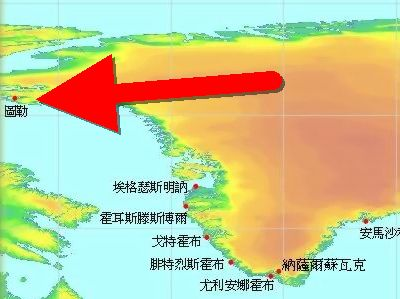
\includegraphics[width=7cm]{圖勒.jpg}

\section*{The End}
\end{document}
